\documentclass[11pt,a4paper]{article}
\usepackage[T1]{fontenc}
\usepackage[utf8]{inputenc}
\usepackage{lmodern}
\usepackage{microtype}
\usepackage{amsmath,amssymb,amsfonts,amsthm,amscd,mathtools}
\usepackage{geometry,graphicx,booktabs,array,enumitem}
\usepackage{tikz,tikz-cd}
\usetikzlibrary{arrows.meta,positioning,calc,patterns}
\usepackage{hyperref}
\usepackage{xcolor}
\geometry{left=2.10cm,right=2.10cm,top=2.00cm,bottom=1.75cm}
\hypersetup{colorlinks=true,linkcolor=blue!45!black,urlcolor=blue!55!black,pdftitle={Brief on Correlations of Sapiens: A Toy Mathematical Framework}}
\setlist[itemize]{topsep=3pt,itemsep=2pt}
\setlist[enumerate]{topsep=3pt,itemsep=3pt}
\allowdisplaybreaks[1]
\numberwithin{equation}{section}

\newtheorem{definition}{Definition}[section]
\newtheorem{theorem}[definition]{Theorem}
\newtheorem{lemma}[definition]{Lemma}
\newtheorem{proposition}[definition]{Proposition}
\newtheorem{corollary}[definition]{Corollary}
\theoremstyle{remark}
\newtheorem{example}[definition]{Example}
\newtheorem{remark}[definition]{Remark}
\newtheorem{hypothesis}[definition]{Hypothesis}

% Retained and regularized shorthand from the original manuscript.
\newcommand{\R}{\mathbb{R}}
\newcommand{\Q}{\mathbb{Q}}
\newcommand{\Z}{\mathbb{Z}}
\newcommand{\Prob}{\mathbb{P}}
\newcommand{\ProbSpace}{\mathsf{Prob}}
\newcommand{\cl}{\operatorname{cl}}
\newcommand{\D}{\mathbf{D}}
\newcommand{\Pow}{\mathcal{P}}
\newcommand{\G}{\mathcal{G}}
\newcommand{\A}{\mathcal{A}}
\newcommand{\X}{\mathcal{X}}
\newcommand{\C}{\mathcal{C}}
\newcommand{\K}{\mathcal{K}}
\newcommand{\1}{\mathbf{1}}
\newcommand{\Hom}{\operatorname{Hom}}
\newcommand{\im}{\operatorname{im}}
\newcommand{\rank}{\operatorname{rank}}
\newcommand{\KL}{\operatorname{D}_{\mathrm{KL}}}
\newcommand{\id}{\operatorname{id}}

\title{\textbf{Brief on Correlations of Sapiens}\\[3pt]
\large A Formal Toy Theory of Labels, Geometry, Dynamics, and Affinity}
\author{666}
\date{13 October 2026\\[5pt]\small Completed mathematical edition: 14 October 2026}

\begin{document}
\maketitle
\begin{abstract}
We develop a deliberately schematic mathematical language for describing
labels, presentation, contextual transformations, and directed relationships
between abstract agents.  The point is to distinguish statements that follow
from axioms from statements that require observations, semantics, or ethical
judgments.  After constructing an agent space, we prove a non-identifiability
lemma, characterize when two social transformations commute, model
four-agent and $n$-agent affinity networks by flag complexes, study a growing
vocabulary of labels, and state conditional results concerning durable mutual
affinity and conservation under social mixing.  The theory is an exercise in
formal modeling: none of its discrete encodings purports to classify actual
human sex, gender, or relationships exhaustively.
\end{abstract}
\tableofcontents

\section{Scope, conventions, and the agent space}

The original expression
\begin{equation}\label{eq:original-skeleton}
\mathrm{agent}:=\bigl(\mathrm{sex}\in2^{\{0,1\}},\
\mathrm{gender}\in2^{\mathit S},\
\mathrm{geometry}\subset\widehat S\bigr)
\end{equation}
is best interpreted as a \emph{typed schematic definition}, not as a
statement about the number or nature of human categories.  We now assign
precise types to all three coordinates.

\begin{definition}[Abstract agent]\label{def:agent}
Fix the following mathematical data:
\begin{enumerate}[label=(\roman*)]
\item a finite \emph{code alphabet} $E=\{0,1\}$ and its power set
      $B=2^E=\{\varnothing,\{0\},\{1\},\{0,1\}\}$;
\item a nonempty set $\G$ of descriptive tags, with label configurations
      $\A=2^{\G}=\Pow(\G)$;
\item a nonempty smooth manifold $M$ (possibly with boundary), used solely
      as an abstract space of observable \emph{presentation coordinates}.
\end{enumerate}
The \emph{agent space} and its projection maps are
\begin{equation}\label{eq:agent-space}
\boxed{\X:=B\times\A\times M,\qquad
x=(b,A,p),\qquad \pi_B(x)=b,\ \pi_\A(x)=A,\ \pi_M(x)=p.}
\end{equation}
\end{definition}

In particular, $|B|=4$ is a theorem about this \emph{encoding}.
It is not a theorem that biological sex has precisely four states.
Similarly, a tag in $\G$ is a symbol supplied by the modeler, not an
objective diagnosis or an exhaustive description of personal identity.
The power set permits multiple tags or no tags; it does not impose a
binary taxonomy on gender.

\begin{remark}[Context is a separate variable]
A relationship or observation generally depends on context $c\in\C$,
where $\C$ may encode time, social setting, communication history, and
sampling conditions.  We do not conflate $c$ with the intrinsic
coordinates of $x$.  An optional fuller state is $(x,c)\in\X\times\C$.
\end{remark}

\subsection{Topology and the correction to the surface analogy}
Give $B$ the discrete topology.  If $\G$ is finite, give $\A$ the
discrete topology as well, and equip $\X$ with the product topology.
If $\G$ is infinite, identify $2^{\G}$ with $\{0,1\}^{\G}$ and equip
it with the product topology.  Neither construction requires the
ill-typed quotient/exponent appearing in the preliminary notes.

Alternatively, when uncertainty about an \emph{observer's assignment}
of tags is of interest, one may introduce a probability distribution
$q\in\ProbSpace(\G)$ and the usual weak topology on the space of probability
measures.  For finite $\G$ this is simply the Euclidean topology on
the probability simplex
\begin{equation}
\Delta(\G)=\left\{(q_g)_{g\in\G}:q_g\ge0,
\ \sum_{g\in\G}q_g=1\right\}.
\end{equation}
Such a $q$ models epistemic uncertainty; it need not represent an
individual's identity as a mixture.

The preliminary ``five-hole torus'' language can be made precise as a
\emph{chosen example}, not a universal model of anatomy or identity.
For the compact orientable surface $\Sigma_{g,r}$ of genus $g$ with $r$
boundary components,
\begin{equation}\label{eq:euler}
\chi(\Sigma_{g,r})=2-2g-r.
\end{equation}
Thus $\chi(\Sigma_{1,5})=-5$, whereas $\chi(S^2)=2$.
The two surfaces are not homeomorphic.  Moreover, \emph{homotopy},
\emph{homeomorphism}, \emph{diffeomorphism}, and a \emph{group action}
are distinct notions; the expression $H\sim f_a$ defines none of them.
No assertion about a ``blow-up'' or non-immersibility follows from
\eqref{eq:euler}.

\section{Transformations, morphisms, and label changes}

\begin{definition}[Contextual action]
A contextual transformation is a specified map
$f_c:\X\to\X$ for $c\in\C$.  A family of such maps is a monoid action
only when there is a monoid $(\C,\circ,e)$ for which
\begin{equation}\label{eq:action}
f_e=\id_\X,\qquad f_{c\circ d}=f_c\circ f_d.
\end{equation}
A group action additionally requires invertible transformations.
\end{definition}

For the discrete label component, it is often more appropriate to use
an \emph{admissible transition relation}
\begin{equation}\label{eq:transition}
T_c\subseteq\X\times\X,\qquad x\overset{c}{\longrightarrow}y
\ \Longleftrightarrow\ (x,y)\in T_c,
\end{equation}
because a transition may be one-to-many or may not have an inverse.
The word ``homomorphism'' should be reserved for a specified algebraic
structure and maps preserving its operations; without those choices,
\eqref{eq:transition} supplies arrows, not homomorphisms.

\subsection{Example: the ``Femboy Girl lemma''}

We retain the manuscript's name as a label for a mathematical thought
experiment.  It is not a claim about the attributes of any real group.
Choose distinct tags $g_0,g_1\in\G$, a presentation point $p_0\in M$,
and the same encoding $b_0\in B$ at two states:
\begin{equation}\label{eq:fembg}
\begin{aligned}
x_0&=(b_0,\{g_0\},p_0),\\
x_1&=(b_0,\{g_1\},p_0),\\
x_0&\overset{c}{\longrightarrow}x_1
\quad\text{if }(x_0,x_1)\in T_c.
\end{aligned}
\end{equation}
This repairs the unfinished ``$\equiv$'' in the source.  The symbol
$g_0\to g_1$ describes a \emph{possible modeled transition}; it does
not follow from a visible feature or from the binary code.

\begin{lemma}[Femboy Girl / non-identifiability lemma]\label{lem:fg}
If $|\G|\ge2$, the projection $\pi_M:\X\to M$ is not injective.
In particular, neither the tag configuration nor the code is uniquely
determined by the presentation coordinate.
\end{lemma}
\begin{proof}
Use the states in \eqref{eq:fembg}.  Since $g_0\ne g_1$,
we have $x_0\ne x_1$, but
$\pi_M(x_0)=p_0=\pi_M(x_1)$.  Hence $\pi_M$ is not injective.
The same argument with distinct $b\in B$ proves non-identifiability
of the code from $p$.
\end{proof}

\begin{center}
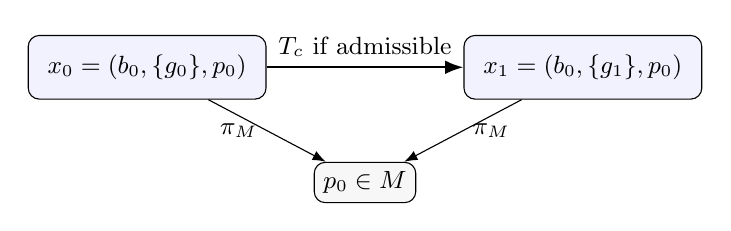
\begin{tikzpicture}[>=Latex, node distance=25mm,
  every node/.style={font=\small}]
\node[draw,rounded corners,fill=blue!5,inner sep=7pt] (a)
  {$x_0=(b_0,\{g_0\},p_0)$};
\node[draw,rounded corners,fill=blue!5,inner sep=7pt,right=of a] (b)
  {$x_1=(b_0,\{g_1\},p_0)$};
\node[draw,rounded corners,fill=gray!6,below=12mm of $(a)!0.5!(b)$]
  (p) {$p_0\in M$};
\draw[->,thick] (a) -- node[above] {$T_c$ if admissible} (b);
\draw[->] (a) -- node[left] {$\pi_M$} (p);
\draw[->] (b) -- node[right] {$\pi_M$} (p);
\end{tikzpicture}
\end{center}

\begin{remark}[On ``more homomorphisms'']
Allowing more arrows in $T_c$ increases the number of \emph{admissible
transitions} by definition.  It does not establish that some real-life
social class possesses more homomorphisms, nor that such transitions
must occur.  This distinction prevents a formal conclusion from being
smuggled in as an empirical premise.
\end{remark}

\section{Correlations in the probabilistic sense}

Let $(\Omega,\mathcal F,\mu)$ be a probability space and
$X=(B_*,A_*,P_*)$ an $\X$-valued random variable.
The statistical relationship between the coordinate variables is
encoded in their \emph{joint law}, not merely in the product
$B\times\A\times M$.

For finite $B,\A$, write
\begin{equation}
p_{bA}=\Prob(B_*=b,A_*=A),\quad
p_b=\sum_Ap_{bA},\quad p_A=\sum_bp_{bA}.
\end{equation}
The mutual information (in nats) is
\begin{equation}\label{eq:mi}
I(B_*;A_*)=
\sum_{\substack{b,A\\p_{bA}>0}}
 p_{bA}\log\frac{p_{bA}}{p_bp_A}
=\KL\!\bigl(\mu_{B_*A_*}\,\|\,\mu_{B_*}\otimes\mu_{A_*}\bigr)
\ge0.
\end{equation}
Equality holds exactly when the two discrete variables are independent.
This is a consequence of the nonnegativity of relative entropy.

\begin{example}[A two-code, two-tag toy distribution]
Suppose a distribution is concentrated on two code values and two tag
configurations, with joint table
\begin{center}
\begin{tabular}{c|cc|c}
 & $A_0$ & $A_1$ & marginal\\\hline
$b_0$ & $0.4$ & $0.1$ & $0.5$\\
$b_1$ & $0.1$ & $0.4$ & $0.5$\\\hline
marginal & $0.5$ & $0.5$ & $1$
\end{tabular}
\end{center}
Then
\begin{equation}
I(B_*;A_*)=0.8\log(1.6)+0.2\log(0.4)
\approx0.192745\ \text{nats}.
\end{equation}
This numerical correlation is a property of the assumed table; it
proves neither a causal link nor a universal correlation in humans.
\end{example}

If $P_*$ takes values in a continuous manifold, correlations involving
its law can likewise be studied using conditional distributions or
relative entropy when the required measures are defined.  There is no
general scalar ``correlation of geometry'' without a chosen statistic.

\section{Directed affinity, reciprocity, and commutativity}

Take $n\ge2$ agents $x_1,\ldots,x_n\in\X$.
For a fixed time $t$ and context $c$, define a directed affinity matrix
\begin{equation}\label{eq:W}
W(t,c)=(w_{ij}(t,c))_{1\le i,j\le n},\quad
w_{ij}\in[0,1],\quad w_{ii}=0.
\end{equation}
The entry $w_{ij}$ is a modeling input, \emph{not} a measured quantity
until an actual measurement protocol is specified.
Let $a_{ij}(t,c)\in\{0,1\}$ denote whether $i$ has granted the particular
modeled interaction toward $j$; neither affinity nor mutuality overrides
this separate consent variable.  Set
\begin{equation}\label{eq:reciprocal}
r_{ij}(t,c)=a_{ij}a_{ji}\min\{w_{ij},w_{ji}\}.
\end{equation}
Then $r_{ij}=r_{ji}$ even when $w_{ij}\ne w_{ji}$.

\begin{lemma}[Conditional commutativity of independent changes]
Suppose $F:U\to U$ and $H:V\to V$ are maps.  Define
$\widetilde F(u,v)=(F(u),v)$ and
$\widetilde H(u,v)=(u,H(v))$ on $U\times V$.
Then
\begin{equation}\label{eq:commuting}
\widetilde F\circ\widetilde H
=\widetilde H\circ\widetilde F.
\end{equation}
\end{lemma}
\begin{proof}
Both compositions take $(u,v)$ to $(F(u),H(v))$.
\end{proof}

The source's shorthand ``$[bg,gb]$'' and ``$[gl,bl]$'' has at least two
possible meanings: exchange of labels on a \emph{relationship}, or the
commutator of \emph{transformations}.  These must not be confused.
If a relationship is defined by $r_{ij}$ in
\eqref{eq:reciprocal}, exchanging $i$ and $j$ is symmetric.
For arbitrary changes $F$ and $H$ of the same state, however, no
commutativity theorem is available.

\begin{example}[Noncommuting label permutations]
On the three-state set $\{1,2,3\}$, let $F=(12)$ and $H=(23)$
be transpositions.  Then
\begin{equation}
(F\circ H)(1)=2,\qquad (H\circ F)(1)=3.
\end{equation}
Therefore $F\circ H\ne H\circ F$.  If these are represented by linear
permutation operators, their Lie bracket $[F,H]=FH-HF$ is nonzero.
A group-theoretic commutator, when appropriate, instead uses
$FHF^{-1}H^{-1}$.
\end{example}

\begin{proposition}[Reciprocity is not directed symmetry]
Symmetry of $R=(r_{ij})$ follows from \eqref{eq:reciprocal} for every
$W$ and $a$.  Symmetry of $W$ itself is an independent hypothesis.
\end{proposition}
\begin{proof}
Exchange $i$ and $j$ in \eqref{eq:reciprocal}; both the product
$a_{ij}a_{ji}$ and the minimum are unchanged.
\end{proof}

\section{From four-love to \texorpdfstring{$n$}{n}-love: combinatorial topology}

The topological construction concerns an \emph{affinity network}, not
the intrinsic identity of its vertices.  Suppress $t,c$ and fix a
threshold $\theta\in(0,1]$.
Define the undirected mutual-affinity graph $G_\theta$ by putting
$\{i,j\}$ in its edge set exactly when $r_{ij}\ge\theta$.
Its \emph{clique (flag) complex} is
\begin{equation}\label{eq:flag}
\K_\theta=
\left\{\sigma\subseteq\{1,\ldots,n\}:
\{i,j\}\in E(G_\theta)\text{ for all distinct }i,j\in\sigma
\right\}.
\end{equation}
Every complete $(k+1)$-vertex subgraph becomes a $k$-simplex.

\begin{theorem}[Four-cycle to full four-way clique]\label{thm:four}
Suppose the edge set of $G_\theta$ consists exactly of the cycle
\begin{equation*}
E(G_\theta)=\bigl\{\{1,2\},\{2,3\},\{3,4\},\{4,1\}\bigr\}.
\end{equation*}
Then $\K_\theta$ has
\begin{equation}
H_1(\K_\theta;\Z)\cong\Z,\qquad
\chi(\K_\theta)=0.
\end{equation}
If all six edges are present instead, $\K_\theta$ is a
three-simplex, and
\begin{equation}
H_1(\K_\theta;\Z)=0,\qquad
\chi(\K_\theta)=1.
\end{equation}
\end{theorem}
\begin{proof}
In the first case the flag complex is the one-dimensional cycle
$C_4$, homeomorphic to $S^1$; thus $H_1\cong\Z$ and
$\chi=4-4=0$.  In the second case the clique complex consists of a
full tetrahedron together with all its faces.  A simplex is
contractible, so its first homology vanishes and its Euler
characteristic is $4-6+4-1=1$.
\end{proof}

\begin{center}
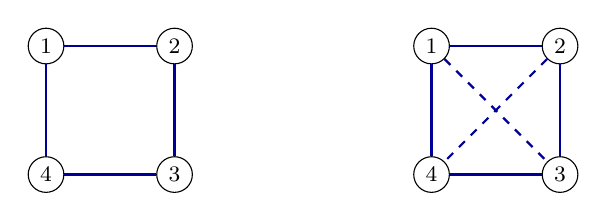
\begin{tikzpicture}[scale=1.02,
 every node/.style={circle,draw,inner sep=2.2pt,font=\footnotesize,fill=white},
 edge/.style={thick,blue!60!black}]
\begin{scope}[xshift=-2.4cm]
\node (a1) at (-.8,.8) {1};\node (a2) at (.8,.8) {2};
\node (a3) at (.8,-.8) {3};\node (a4) at (-.8,-.8) {4};
\draw[edge] (a1)--(a2)--(a3)--(a4)--(a1);
\end{scope}
\begin{scope}[xshift=2.4cm]
\node (b1) at (-.8,.8) {1};\node (b2) at (.8,.8) {2};
\node (b3) at (.8,-.8) {3};\node (b4) at (-.8,-.8) {4};
\draw[edge] (b1)--(b2)--(b3)--(b4)--(b1);
\draw[edge,dashed] (b1)--(b3) (b2)--(b4);
\end{scope}
\end{tikzpicture}

\smallskip
\small $C_4$: a one-dimensional hole \hspace{23mm}
$K_4$: flag complex fills all faces and the interior
\end{center}

\begin{example}[Explicit weights and a topological transition]
Let all consent entries for distinct pairs equal $1$ and take
\begin{equation}\label{eq:W4}
W=\begin{pmatrix}
0&.9&.2&.9\\
.9&0&.9&.2\\
.2&.9&0&.9\\
.9&.2&.9&0
\end{pmatrix}.
\end{equation}
At $\theta=0.8$, only the cycle edges are present, so
$\beta_1=\rank H_1=1$.  At $\theta=0.2$, the two diagonals
enter; all four vertices form a simplex, and $\beta_1=0$.
The abrupt jump occurs in the \emph{thresholded model} and should
not be mistaken for a physical singularity in anyone's emotions.
\end{example}

\begin{proposition}[$n$-cycle versus $n$-clique]
For $n\ge4$, the flag complex of the chordless cycle $C_n$ has
$H_1\cong\Z$ and $\chi=0$.  The flag complex of the complete graph
$K_n$ is an $(n-1)$-simplex and has $H_1=0$ and $\chi=1$.
\end{proposition}
\begin{proof}
A chordless $n$-cycle for $n\ge4$ has no $3$-cliques, hence its flag
complex is homeomorphic to a circle.  A complete graph has every
possible clique and therefore generates a simplex.
\end{proof}

This offers a precise meaning for the manuscript's phrase
``four-love to $n$-love singularities'': critical parameter levels
where the homotopy type or Betti numbers of $\K_\theta$ change.
A genuinely dynamical bifurcation would require a separate equation
of motion and appropriate nondegeneracy assumptions.

\section{Changing vocabularies: the ``Europian'' lemma}

The preliminary notes anticipated future change in the number or
meaning of tags.  We retain ``Europian'' as an internal nickname only;
it has no geographical or sociological content.

\begin{definition}[Vocabulary filtration]
A vocabulary filtration is a sequence of finite sets
\begin{equation}\label{eq:Gfiltration}
\G_0\subseteq\G_1\subseteq\G_2\subseteq\cdots,
\qquad \A_t=2^{\G_t},\qquad \X_t=B\times\A_t\times M.
\end{equation}
The canonical inclusion sends $(b,A,p)\in\X_t$ to the same triple
viewed as an element of $\X_{t+1}$.
\end{definition}

\begin{lemma}[``Europian'' vocabulary-expansion lemma]\label{lem:expansion}
If $|\G_{t+1}|=|\G_t|+k$, the number of possible discrete
label configurations changes by a factor $2^k$:
\begin{equation}\label{eq:expansion}
|\A_{t+1}|=2^k|\A_t|.
\end{equation}
The canonical map $\X_t\hookrightarrow\X_{t+1}$ is injective.
\end{lemma}
\begin{proof}
For a finite set with $m$ elements, its power set has $2^m$
elements.  Inclusion preserves each triple exactly, so distinct
triples remain distinct.
\end{proof}

\begin{remark}[Expansion is not a demographic prediction]
Equation \eqref{eq:expansion} counts formal subsets.  It does not
predict that a population's observed identities will double, or that
adding a term creates a previously nonexistent kind of person.
\end{remark}

A separate issue arises with temporal continuity.  If $\G$ is
finite and label configurations carry the discrete topology, a
continuous curve $A:[0,1]\to2^{\G}$ must be constant: the continuous
image of the connected interval is connected, and connected subsets
of a discrete space are singletons.  Therefore changes of labels
must be modeled using (i) jumps, (ii) a varying vocabulary, or
(iii) an auxiliary continuous epistemic variable $q(t)\in\Delta(\G)$.
This is a mathematical obstruction to the initial informal idea that
a discrete tag system can also vary continuously without modification.

\begin{hypothesis}[Optional social evolution law]
Given row-stochastic matrices $K_t$ indexed by $\A_t$, a probability
row vector $\rho_t$ over label configurations can evolve as
\begin{equation}\label{eq:markov}
\rho_{t+1}=\rho_tK_t,
\quad K_t(A,A')\ge0,
\quad\sum_{A'}K_t(A,A')=1.
\end{equation}
This is an \emph{assumed} Markov model, not a consequence of the agent
space.  If $\G_t$ changes, $K_t$ must be rectangular with the old
and new state spaces as its row and column indices.
\end{hypothesis}

\section{Ideal love as an explicitly conditional definition}

The mathematical system by itself cannot determine what ``true love''
means.  Such a conclusion requires criteria chosen \emph{outside} the
algebra.  We can nevertheless formalize one operational notion of a
stable, mutual, consensual relationship.

\begin{definition}[Stable mutual affinity on an interval]
Fix a threshold $\theta\in(0,1]$ and interval
$I=[t_0,t_0+T]$.  A pair $(i,j)$ is called
$\theta$-stable on $I$ if
\begin{equation}\label{eq:stable}
a_{ij}(t)=a_{ji}(t)=1
\quad\text{and}\quad
\min\{w_{ij}(t),w_{ji}(t)\}\ge\theta
\quad\text{for every }t\in I.
\end{equation}
This is a stipulated criterion, not a psychological or moral theorem.
\end{definition}

\begin{theorem}[A local stability certificate]\label{thm:stability}
Assume consent holds throughout $I$ and both directed affinities are
$L$-Lipschitz in time: for $k\ell=ij,ji$,
\begin{equation}
|w_{k\ell}(t)-w_{k\ell}(s)|\le L|t-s|.
\end{equation}
If $r_{ij}(t_0)\ge\theta+\varepsilon$ for $\varepsilon>0$, then the
pair is $\theta$-stable on every interval
$[t_0,t_0+T]$ with $T\le\varepsilon/L$, provided $L>0$.
If $L=0$, it remains stable for the whole consent interval.
\end{theorem}
\begin{proof}
For $t\ge t_0$, the Lipschitz bounds give
$w_{ij}(t)\ge w_{ij}(t_0)-L(t-t_0)$ and the analogous bound
for $w_{ji}$.  Taking the minimum yields
\begin{equation}
\min\{w_{ij}(t),w_{ji}(t)\}
\ge r_{ij}(t_0)-L(t-t_0)
\ge\theta+\varepsilon-LT\ge\theta.
\end{equation}
Together with the maintained consent assumptions, this proves
\eqref{eq:stable}.
\end{proof}

\begin{remark}[Limits of the certificate]
This is a \emph{sufficient local condition}, not a prediction of
durable relationships.  A withdrawal of consent invalidates the
premise instantly, irrespective of the affinities.  Emotional
well-being, autonomy, honesty, reciprocity, and personal meaning
cannot be established from a scalar $w_{ij}$ without explicit,
independently justified definitions.
\end{remark}

\section{Fuzzy--lazy dating: incomplete data and conservation}

\subsection{Underdetermination is not overdetermination}
In an $n$-agent network there are $d=n(n-1)$ unknown directed
non-diagonal affinities at a fixed time.  Stack them into
$z\in[0,1]^d$.  A simplified observation model is
\begin{equation}\label{eq:inverse}
y=Hz+\eta,\qquad H\in\R^{m\times d},
\end{equation}
where $y$ contains observations and $\eta$ accounts for noise.

\begin{proposition}[Underdetermined observations]
If $\eta=0$, $m<d$, and $H$ has rank $r$, the unconstrained solution
set of $Hz=y$, when nonempty, is an affine space of dimension $d-r$.
If one feasible solution lies in the interior of $[0,1]^d$, there
are infinitely many feasible solutions whenever $r<d$.
\end{proposition}
\begin{proof}
For any particular solution $z_0$, the solutions form
$z_0+\ker H$.  The rank--nullity theorem gives
$\dim\ker H=d-r$.  A sufficiently small neighborhood of an
interior $z_0$ remains inside $[0,1]^d$, so nonzero kernel
directions generate infinitely many feasible points.
\end{proof}

\begin{example}[Three agents with two observations]
For $n=3$ there are six directed variables.  Knowing
$w_{12}=0.8$ and $w_{21}=0.7$ leaves four variables unspecified.
One cannot conclude whether $(2,3)$ is reciprocally linked at
threshold $0.6$.  Thus the unseen part of the network is
\emph{underdetermined}, not ``overdetermined''.
\end{example}

In contrast, an \emph{overdetermined} system has more independent or
redundant measurements than unknown parameters; it may be
inconsistent under noise.  A modeler may then minimize, for example,
\begin{equation}\label{eq:regularized}
\widehat z=\mathop{\arg\min}_{z\in[0,1]^d}
\left\{\frac12\|Hz-y\|_2^2+\frac{\lambda}{2}\|Lz\|_2^2\right\},
\end{equation}
with a specified regularizer $L$ and $\lambda\ge0$.
The regularizer supplies an assumption; it does not magically recover
information absent from $y$.

\subsection{A precise uniform-conservation statement}
Let $u(t)\in\R^n$ describe a generic transferable quantity, such as
attention units in a mathematical allocation model.  (Real human
affection need not obey a conservation law.)  Consider the discrete
evolution
\begin{equation}\label{eq:mixing}
u(t+1)=Pu(t),\qquad P_{ij}\ge0.
\end{equation}

\begin{theorem}[Uniform conservation under doubly stochastic mixing]
If $P$ is \emph{doubly stochastic}, meaning
\begin{equation}\label{eq:doubly}
P\1=\1,\qquad \1^{\mathsf T}P=\1^{\mathsf T},
\end{equation}
then both the total and the uniform mean are invariant:
\begin{equation}\label{eq:conservation}
\boxed{\1^{\mathsf T}u(t)=\1^{\mathsf T}u(0),
\qquad \overline u(t)=\frac1n\sum_{i=1}^nu_i(t)=\overline u(0).}
\end{equation}
\end{theorem}
\begin{proof}
By \eqref{eq:doubly},
$\1^{\mathsf T}u(t+1)=\1^{\mathsf T}Pu(t)=\1^{\mathsf T}u(t)$.
Induction proves total conservation, and dividing by $n$ proves
mean conservation.
\end{proof}

\begin{example}[Why row stochasticity alone is insufficient]
The matrix
\begin{equation}
P=\begin{pmatrix}0.9&0.1\\0.6&0.4\end{pmatrix}
\end{equation}
is row stochastic but not column stochastic.  With
$u(0)=(1,0)^{\mathsf T}$, one obtains
$u(1)=(0.9,0.6)^{\mathsf T}$ and the total increases from $1$
to $1.5$.  Conversely,
$Q=\bigl(\begin{smallmatrix}0.8&0.2\\0.2&0.8\end{smallmatrix}\bigr)$
is doubly stochastic and preserves the total.
\end{example}

\begin{corollary}[Continuous-time network Laplacian]
Let $L$ be a graph Laplacian satisfying
$\1^{\mathsf T}L=0$, and let
$\dot u=-Lu$.  Then $\1^{\mathsf T}u(t)$ is constant.
\end{corollary}
\begin{proof}
Differentiate:
$\frac{d}{dt}(\1^{\mathsf T}u)
=-\1^{\mathsf T}Lu=0$.
\end{proof}

\section{Synthesis: what can and cannot be derived}

The formal dependencies in this paper can be summarized as
\begin{equation}\label{eq:dependency}
\begin{gathered}
(B,\G,M)\longrightarrow\X
\longrightarrow\bigl(\text{state maps},\ \text{observations}\bigr),\\
(W,a,\theta)\longrightarrow G_\theta
\longrightarrow\K_\theta
\longrightarrow H_k(\K_\theta),\\
\text{extra dynamical axioms}\longrightarrow
\text{conditional stability and conservation statements}.
\end{gathered}
\end{equation}
The arrows in \eqref{eq:dependency} record logical dependence, not
causal relationships in the world.

\begin{enumerate}[label=\textbf{\arabic*.}]
\item A finite code or vocabulary gives a combinatorial state count.
      Its semantic completeness is \emph{not} guaranteed.
\item Presentation need not identify labels.  This is a precise
      non-injectivity assertion, not a psychological theory.
\item Affinity symmetry may be imposed by reciprocal aggregation;
      unrestricted transformations need not commute.
\item The topology of a thresholded graph can change with the
      threshold, giving a legitimate but model-dependent notion of
      ``singularity.''
\item Evolving vocabularies produce an inclusion system, not
      independently verifiable forecasts of social development.
\item ``Ideal love'' requires chosen criteria, and stability follows
      only under maintained assumptions such as consent and a
      Lipschitz bound.
\item Incomplete observations produce non-identifiability.
      Conservation requires a specific evolution operator.
\end{enumerate}

\paragraph{Conclusion.}
The useful mathematical core is not a purported classification of
\emph{Homo sapiens}; it is the separation of \emph{types, topology,
observations, dynamics, and proofs}.  Once these are distinguished,
several formerly speculative statements become valid conditional
lemmas.  The remaining claims should be regarded as questions about
empirical modeling, meaning, and values rather than deductions from
symbolic notation.

\appendix
\section{Notation and types}
\begin{center}
\renewcommand{\arraystretch}{1.12}
\begin{tabular}{@{}p{.21\textwidth}p{.70\textwidth}@{}}
\toprule
Symbol & Mathematical meaning\\
\midrule
$E,\ B=2^E$ & Two-symbol alphabet and its four-element power set; formal encoding only.\\
$\G,\ \A=2^\G$ & Tag vocabulary and allowable subsets of tags.\\
$M,\ \X$ & Presentation manifold and product agent space $B\times\A\times M$.\\
$\C,\ f_c,\ T_c$ & Contexts; specified state maps; permitted state transitions.\\
$\chi,\ H_k$ & Euler characteristic and singular homology groups.\\
$W=(w_{ij})$ & Directed, context-dependent affinity weights in $[0,1]$.\\
$a_{ij},\ r_{ij}$ & Consent indicator and symmetrized mutual-affinity score.\\
$G_\theta,\ \K_\theta$ & Threshold graph and its clique/flag complex.\\
$\G_t,\ \rho_t,\ K_t$ & Time-indexed vocabulary, probability law, and stochastic evolution kernel.\\
$H,z,y$ & Observation matrix, unknown affinity vector, and observed data.\\
$P,L,u$ & Mixing matrix, network Laplacian, and generic conserved-state vector.\\
\bottomrule
\end{tabular}
\end{center}

\section{Open questions for a genuinely empirical extension}
A future empirical study would first need a defensible sampling frame,
operational definitions of every recorded feature, consent to collect
sensitive observations, uncertainty calibration, and a pre-specified
statistical objective.  Only then would questions such as the
following be testable:
\begin{enumerate}
\item Which finite-dimensional features, if any, are adequate for a
      particular prediction task, and with what generalization error?
\item Does a chosen social transition kernel fit longitudinal
      observations better than a static baseline?
\item How sensitive are topological summaries of affinity networks
      to measurement noise and the threshold $\theta$?
\item Under which conditions is a proposed stability measure
      robust to missing data, time variation, and asymmetric reports?
\item Can one test a conservation law against observations, rather
      than imposing it through a doubly stochastic transition matrix?
\end{enumerate}
No empirical answers are assumed.

\end{document}
